\chapter{Computational Details}
This chapter provides the details of the computational methods used in this work. The first section describes the generation of the training dataset, including the preparation of the system, initial equilibration using the molecular mechanics, exploration of the configuration space at the xTB level, further data labeling, and iterative training of the neural network potential. The second section discusses the production runs at different temperatures using the fitted neural network potential. The third section describes the workflow of validating the transition states obtained from the simulations following the partial Hessian formalism. Finally, the fourth section presents the data analysis and visualisation techniques employed to interpret the results.



\section{Training dataset generation}



\subsection{System preparation}
The systems were prepared using the CHARMM-GUI webserver's functionality \citep{jo_charmm-gui_2008}. In particular, the Multicomponent Assembler interface \citep{kern_charmm-gui_2024} was utilised. 

As a first step, the singly protonated and deprotonated forms of the methyl diphosphate were parametrised in CGenFF \citep{kim_charmm-gui_2017}, i.e. CHARMM General Forcefield. These states of the methyl diphosphate were chosen based on the fact that pyrophosphoric (diphosphoric) acid has the following dissociation constants \citep{haynes_crc_2016}:
\begin{align*}
    \mathrm{H_4P_2O_7} \rightleftharpoons \mathrm{[H_3P_2O_7]^-} + \mathrm{H^+},\quad \mathrm{p}K_\mathrm{a} = 0.91 \\
    \mathrm{[H_3P_2O_7]^-} \rightleftharpoons \mathrm{[H_2P_2O_7]^{2-}} + \mathrm{H^+},\quad \mathrm{p}K_\mathrm{a} = 2.10 \\
    \mathrm{[H_2P_2O_7]^{2-}} \rightleftharpoons \mathrm{[HP_2O_7]^{3-}} + \mathrm{H^+},\quad \mathrm{p}K_\mathrm{a} = 6.70 \\
    \mathrm{[HP_2O_7]^{3-}} \rightleftharpoons \mathrm{[P_2O_7]^{4-}} + \mathrm{H^+},\quad \mathrm{p}K_\mathrm{a} = 9.32
\end{align*}
Thus, at the physiological pH of 7.4 this acid exists as an equillibrium between the doubly and singly protonated forms. As an assumption, the methyl group can be considered as a proton, therefore we condsidered the methyl diphosphate molecule to exist as a mixture of the singly (MeHDP) and deprotonated (MeDP) forms at the physiological pH.

After succesfully parametrising the molecules, the system was solvated in a cubic box of TIP3 water molecules together with the sodium counterions Na\textsuperscript{+} to neutralise the charge. The final system composition can be seen in Table \ref{tab:system-before-equilibration}.

\subsection{Initial equilibration using the classical forcefields}
The equilibration of the system was performed following the standard protocol generated by the CHARMM-GUI webserver \citep{jo_charmm-gui_2008}. The system was first energy minimised using the steepest descent algorithm for 5000 steps. 

Subsequently the system was equillibrated in the NVT (constant number of particles, volume, and temperature) ensemble for 5 ns. During the minimisation and NVT equilibration, the heavy atoms of the solute were restrained using a harmonic potential with a force constant of 400 kJ mol\textsuperscript{-1} nm\textsuperscript{-2}.

As a last step, the system was equilibrated in the NPT (constant number of particles, pressure, and temperature) ensemble for 45 ns. Throughout the whole protocol, the temperature was set to 300 K and the pressure was set to 1 bar. To ensure the constant temperature and pressure, the system was coupled to a $\nu$-rescale thermostat with a coupling constant of 1 ps and an isotropic \textit{c}-rescale barostat with a coupling constant of 5 ps. During the NPT run, the cut-off for the non-bonded interactions was set to 0.6 nm and the long-range electrostatics were treated using the Particle Mesh Ewald (PME) method.

All simulations were conducted in GROMACS 2021.4 \citep{abraham_gromacs_2015} using the CHARMM36m forcefield \citep{huang_charmm36m_2017} and the leap-frog integration method with a time step of 1 fs. All hydrogen involving bonds were constrained using the LINCS algorithm. The final dimensions of the box for all further calculations were obtained after the NPT run and are shown in Table \ref{tab:system-before-equilibration}.
\begin{table}[htbp]
    \centering
    \caption{System composition and simulation box details. \textsuperscript{1}The final dimensions were obtained after the NPT run using the CHARMM36m forcefield.}
    \label{tab:system-before-equilibration}
    \begin{tabular}{@{}lccc@{}}
    \toprule
    System & Equillibrated box dimensions\textsuperscript{1} (\AA) & No. of water molecules & No. of Na\textsuperscript{+} \\
    \midrule
    MeDP  & $15.877 \times 15.877 \times 15.877$ & 119 & 3 \\
    MeHDP & $15.901 \times 15.901 \times 15.901$ & 124 & 2 \\
    \bottomrule
    \end{tabular}
\end{table}



\subsection{GFN1-xTB based exploration of the configuration space}
To generate the first set of the configurations for the training dataset, the system was subjected to molecular dynamics simulations using the semi-empirical GFN1-xTB \citep{grimme_robust_2017} level of theory. GFN1-xTB gives a good first approximation of the potential energy surface and is computationally efficient hence making it suitable for relatively long MD simulations of big systems. 

Each system was first equilibrated for 5 ps in the NVT ensemble at 300 K to relax the structures at the GFN1-xTB level of theory with a D3 dispersion correction \citep{grimme_consistent_2010}. Afterwards, we performed 50 ps long well-tempered metadynamics (WTMD) simulations in the NVT ensemble as well. In the latter simulation, the biasing potential was applied to force the system to explore the configuration space outside of the reactants basin. The biasing potential was added along two collective variables: the distance between the $\beta$-phosphorus and the oxygen atom connecting it to the rest of the molecule and the coordination number of water oxygens around the $\beta$-phosphorus atom. The more information on the collective variables matter will be provided in the next section. 

All calculations were performed using the CP2K 2023.1 package \citep{kuhne_cp2k_2020}. The temperature was controlled by means of the velocity-rescaling thermostat \citep{bussi_canonical_2007} with a time constant of 50 fs for the equillibration and 100 fs for the WTMD run. The SCF convergence was set to $10^{-5}$ a.u. The biasing potential was applied every 25 fs with a gaussian hill height of 2 kcal mol\textsuperscript{-1} and a width of 0.07 for each CV. The bias factor was set to 30. Lastly, the time step for the integration was set to 0.5 fs. Throughout all simulations, the periodic boundary conditions (PBC) were applied in all directions.



\subsection{Collective variables}

\subsection{Data labeling}

\subsection{Iterative training of the neural network potential}

\subsubsection{First round}

\subsubsection{Second round}

\subsubsection{Third round}
\begin{figure}[h]
    \centering
    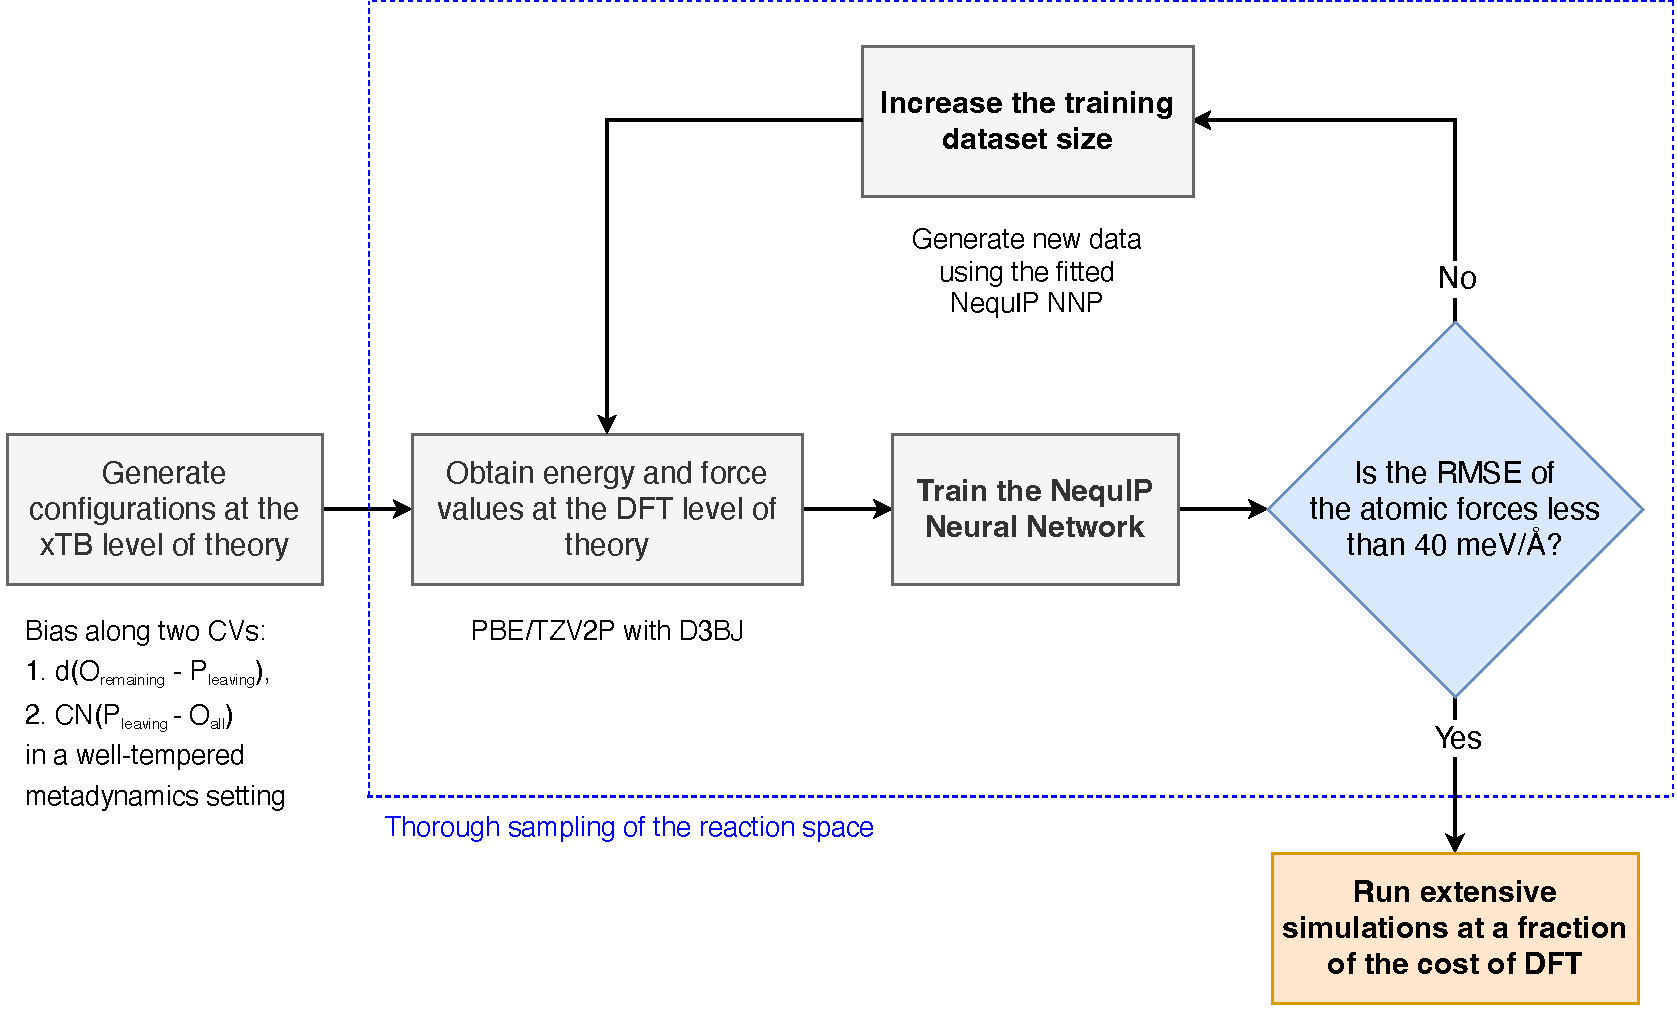
\includegraphics[width=0.95\textwidth]{Figures/3_Computational_details/workflow_diagram_helvetica_updated.pdf}
    \caption{The iterative training of the NequIP neural network potential.}
    \label{fig:iterative-training}
\end{figure}


\section{Production runs at different temperatures}



\section{Validation of the transition states}



\section{Data analysis and visualisation}